% Copyright 2009 by Tomasz Mazur
%
% This file may be distributed and/or modified in all ways.

%\documentclass[xcolor=pdftex,t,11pt]{beamer}
\documentclass[xcolor=pdftex,t,11pt,handout]{beamer}

%%%%%%%%%%%%%%%%%%%%%%%%%%%%%%%%%%
%       SET OPTIONS BELOW        %
%%%%%%%%%%%%%%%%%%%%%%%%%%%%%%%%%%
\usepackage[icelandic, english]{babel}
\usepackage{t1enc} 
\usepackage{textcomp}
\usepackage[
% Toggle showing page counter
pagecounter=true,
%
% String to be used between the current page and the
% total page count, e.g. of, /, from, etc.
pageofpages=of,
%
% Defines the shape of bullet points. Available options: circle, square
bullet=circle,
%
% Show a line below the frame title. 
titleline=true,
%
% Set the style of the title page (true for fancy, false for standard)
alternativetitlepage=true,
%
% Institution logo for fancy title page.
% Comment out to remove the logo from the title page.
% IMPORTANT: THERE IS A BUG IN SOME VERSIONS OF PDFLATEX AND FONTS
% ON THE LOGOS ARE NOT RENDERED PROPERLY. IN SUCH A CASE ADD `2` 
% TO THE NAME OF THE LOGO, E.G. comlab2 INSTEAD OF comlab
titlepagelogo=../hilogo,
%
% Department footer logo for fancy title page
% Comment out to remove the logo from the footer of the title page/
% IMPORTANT: THERE IS A BUG IN SOME VERSIONS OF PDFLATEX AND FONTS
% ON THE LOGOS ARE NOT RENDERED PROPERLY. IN SUCH A CASE ADD `2` 
% TO THE NAME OF THE LOGO, E.G. comlab2 INSTEAD OF comlab
%titlepagefooterlogo=images/titlepage/comlab,
%
% Institution/department logo for ordinary slides
% Comment this line out to remove the logo from all the pages.
% Available logos are: ou, comlab, comlabinline, comlabou
% IMPORTANT: THERE IS A BUG IN SOME VERSIONS OF PDFLATEX AND FONTS
% ON THE LOGOS ARE NOT RENDERED PROPERLY. IN SUCH A CASE ADD `2` 
% TO THE NAME OF THE LOGO, E.G. comlab2 INSTEAD OF comlab
ordinarypageslogo=../hilogoname,
%
%
% Add watermark in the bottom right corner
%watermark=<filename>,
%
% Set the height of the watermark.
%watermarkheight=100pt,
%
% The watermark image is 4 times bigger than watermarkheight.
%watermarkheightmult=4,
]{../beamerthemeTorino} 

% Select color theme. Available options are:
% mininmal, greenandblue, blue, red
\usepackage{../beamercolorthemehi}

%Select different font themes.Available options are:
% default, serif, structurebold, structureitalicserif, structuresmallcapsserif
\usefonttheme{structurebold}

\setbeamercovered{transparent}

%\usepackage{epsfig}
%\usepackage{subfigure}
%\usepackage{calc}
%\usepackage{amssymb}
%\usepackage{amstext}
%\usepackage{amsmath}
%\usepackage{amsthm}
%\usepackage{multicol}
%\usepackage{pslatex}
%\usepackage{apalike}
%\usepackage{SCITEPRESS}
%\usepackage[small]{caption}
\usepackage{booktabs}



\usepackage{url}
\usepackage{subfigure}
% Use graphicx for including graphics
%\usepackage[dvips]{graphicx,psfrag}
\usepackage{graphicx}
\usepackage{paralist}
\usepackage{epstopdf}
\usepackage{natbib} %citep and citet
%\bibpunct[:]{(}{)}{;}{a}{}{,}
%\renewcommand{\bibsection}{\subsubsection*{\bibname } }

%\usepackage[inline]{enumitem} - looses bullet function :S

\newcommand{\bi}{\begin{itemize}\item}
\newcommand{\ei}{\end{itemize}}

\usepackage{latexsym}
\usepackage{amsmath,bm,amssymb}

\usepackage[colorinlistoftodos]{todonotes}
\usepackage{comment}
\usepackage{multirow}
\usepackage{rotating}
\usepackage{longtable}
\usepackage{paralist}
\usepackage[perpage,symbol*]{footmisc}
\usepackage{tabu}
\usepackage{tabularx}
\newcommand{\tcr}[1]{{\color{red} #1}}
\newcommand{\tcb}[1]{{\color{blue} #1}}
\newcommand{\tcg}[1]{{\color{green} #1}}

\usepackage{paralist}


%\renewcommand{\rho}{{\varrho}}

\renewcommand{\vec}[1]{\mathbf{#1}}
\newcommand{\vphi}{{\boldsymbol{\phi}}}
\newcommand{\Exp}{{\mathbb E}}
\newcommand{\inner}[2]{\big<{#1}\cdot{#2}\big>}
\newcommand{\norm}[1]{\lVert#1\rVert}

\newcommand{\vsigma}{{\vec{\sigma}}}
\newcommand{\mat}[1]{\mathbf{#1}}
\newcommand{\R}{{\mathbb R}}
\newcommand{\strng}[1]{{\mbox{\tt #1}}}
\newcommand{\abs}[1]{\lvert#1\rvert}
\newcommand{\argmax}{\mathop{\rm argmax}}
\newcommand{\argmin}{\mathop{\rm argmin}}


\hyphenpenalty=750
\hyphenation{heur-ist-ics}
\hyphenation{algo-rithm}

% job-related
\newcommand{\phiproc}{$\phi_1$}
\newcommand{\phistartTime}{$\phi_2$}
\newcommand{\phiendTime}{$\phi_3$}
\newcommand{\phiwrmJob}{$\phi_4$}
\newcommand{\phiwait}{$\phi_5$}
\newcommand{\phiarrivalTime}{$\phi_6$}
\newcommand{\phijobOps}{$\phi_7$}
% mac-related
\newcommand{\phimac}{$\phi_8$}
\newcommand{\phimacFree}{$\phi_9$}
\newcommand{\phiwrmMac}{$\phi_{10}$}
\newcommand{\phimacOps}{$\phi_{11}$}
% flow-related
\newcommand{\phislotCreated}{$\phi_{12}$}
\newcommand{\phislotReduced}{$\phi_{13}$}
\newcommand{\phislots}{$\phi_{14}$}
\newcommand{\phislotsTotal}{$\phi_{15}$}
% schedule related
\newcommand{\phimakespan}{$\phi_{16}$}
\newcommand{\phiwrmTotal}{$\phi_{17}$}
\newcommand{\phitotProc}{$\phi_{18}$}
\newcommand{\phistep}{$\phi_{19}$}
% global
\newcommand{\phiMWR}{$\phi_{20}$}
\newcommand{\phiLWR}{$\phi_{21}$}
\newcommand{\phiSPT}{$\phi_{22}$}
\newcommand{\phiLPT}{$\phi_{23}$}
\newcommand{\phiRND}{$\phi_{24}$}


\usepackage{cleveref} % must come last! 
 % put your own shorthand declarations in this document

\graphicspath{{../../LION09/figures/},{figures/}}
\DeclareGraphicsExtensions{.eps}
%%%%%%%%%%%%%%%%%%%%%%%%%%%%%%%%%%
%       PRESENTATION INFO        %
%%%%%%%%%%%%%%%%%%%%%%%%%%%%%%%%%%
\author{Helga Ingimundard\'{o}ttir\\Thomas Philip Runarsson}
\title{Generating Training Data for Learning Linear \\ Composite Dispatching Rules for Scheduling}
\institute{University of Iceland}	
\date{January, 2015}


\begin{document}


%%%%%%%%%%%%%%%%%%%%%%%%%%%%%%%%%%
%       SLIDE DEFINITIONS        %
%%%%%%%%%%%%%%%%%%%%%%%%%%%%%%%%%%

\begin{frame}[plain]
	\titlepage
\end{frame}

\frame{
\frametitle{Outline}
\tableofcontents[part=0] % part=0, sectionstyle=show/shaded
}

\section{Introduction}
\frame{\tableofcontents[currentsection]}

\frame{
\frametitle{Motivation}

\begin{block}{General Goal}
\begin{itemize} 
\item General goal is how to search for \emph{good} solutions for an arbitrary problem domain. 
\item Automate the design of optimization algorithms. 
\item Use of randomly sampled problem instances and their corresponding optimal vs. suboptimal solutions.
\end{itemize}
\end{block}
}

\frame{\frametitle{Case Study: JSP}
\begin{block}{Abstract}	
\begin{itemize}
\item Framework for creating dispatching rules for JSP.
\item \alert{Linear classification} to identify good dispatches from worse ones.
\item Generate training data both from \alert{optimal} and \alert{suboptimal} solutions, by exploring various \alert{trajectories} within the state-space.
\item Sample training data using different \alert{ranking} schemes.
\end{itemize}
\end{block}
\textbf{Keywords:} Scheduling $\bullet$ Composite dispatching rules $\bullet$ JSP  $\bullet$ Generating Training Data $\bullet$  Trajectory Sampling Strategies $\bullet$ Ranking Schemes }


\section{Job Shop Scheduling}
\frame{\tableofcontents[currentsection]}

\frame[allowframebreaks]{
\frametitle{Job Shop Scheduling}
\begin{block}{JSP}
	Simple job shop scheduling problem  is where $n$ jobs are scheduled on a set of $m$ machines, subject to constraints:
	\begin{itemize}
	\item each job must follow a predefined machine order,
	\item that a machine can handle at most one job at a time.
	\end{itemize}
	
	\textbf{Objective:} schedule the jobs so as to minimize the maximum completion time, i.e., makespan, $C_{\max}$.
\end{block}
%\begin{itemize}
%	\item Job $j$ has an indivisible operation time on machine $a$, $p(j,a)$, which is assumed to be integral, where $j \in\{1,..,n\}$ and $a\in\{ 1,..,m\}$. 
%	\item Job $j$ has a specified processing order through the machines, it is a permutation vector, $\sigma_j$, of $\{1,..,m\}$, i.e. $j$ can be processed on $\sigma_j(a)$ only after it has completed on $\sigma_j(a-1)$.
%	\begin{itemize} \item Permutation flow shop scheduling (PFSP) is when $\sigma_j$ is fixed $\forall j$. \end{itemize}
%\end{itemize}

\framebreak
\begin{block}{Problem space distributions used in experimental studies}
\begin{table}
{
\begin{tabularx}{\columnwidth}{ll|c|C|C|l}\toprule
&name&size & $N_{\text{train}}$&$N_{\text{test}}$  & note 
\\  \midrule
\multirow{2}{*}{\begin{sideways}JSP\end{sideways}}
&$\mathcal{P}_{j.rnd}^{6\times5}$ & $6\times5$ & 500 & 500 & random \\
&$\mathcal{P}_{j.rndn}^{6\times5}$ & $6\times5$ & 500 & 500 & random-narrow \\
\bottomrule
\end{tabularx}
}\end{table}
\end{block}

\framebreak
\begin{block}{Dispatching rules (DR) for constructing JSP}
\begin{itemize}
	\item Starts with an empty schedule and adds on one job at a time. 
	\item When a machine is free the DR inspects the waiting/available jobs and selects the job with the \alert{highest priority}. 
	\item Complete schedule consists of $\ell=n\cdot m$ sequential dispatches.
	\item At each dispatch $k$, \alert{features} $\vphi(k)$ for the temporal schedule are calculated.
	\item Performance of DR is compared with its optimal makespan, as percentage relative deviation from optimality: $\rho=\frac{C_{\max}^{DR}-C_{\max}^{opt}}{C_{\max}^{opt}}\cdot 100\%$
\end{itemize}
\end{block}
\framebreak
\begin{block}{Features for JSP}\label{tbl:features}
\begin{table}[t!]
 {\scriptsize
 \begin{center}
  \begin{tabular}{|c|l|}
   \hline\hline
  $\vphi$ & Feature description \\ \hline
  $\phi_1$ & processing time for job on machine\\
  $\phi_2$ & start-time \\
  $\phi_3$ & end-time \\
  $\phi_4$ & when machine is next free \\
  $\phi_5$ & current makespan \\
  $\phi_6$ & work remaining \\
  $\phi_7$ & most work remaining \\
  $\phi_8$ & slack time for this particular machine \\
  $\phi_9$ & slack time for all machines \\
  $\phi_{10}$ & slack time weighted w.r.t. number of operations already assigned \\
  $\phi_{11}$ & time job had to wait\\
  $\phi_{12}$ & size of slot created by assignment \\
  $\phi_{13}$ & total processing time for job \\
 \hline\hline
  \end{tabular}
 \end{center}}
\end{table}
\end{block}

\framebreak
\begin{example}
	\begin{center}
		\includegraphics[width=0.5\columnwidth]{jssp_example_nocolor.pdf}
	\end{center}
	A schedule being built at step $k=16$. The dashed boxes represent five different possible jobs that could be scheduled next using a DR.
\end{example}
}

\frame[allowframebreaks]{\frametitle{Game-tree representation}
	\begin{example}{First layer (i.e. root) -- empty schedule at step $k=1$}
		\begin{figure} \centering 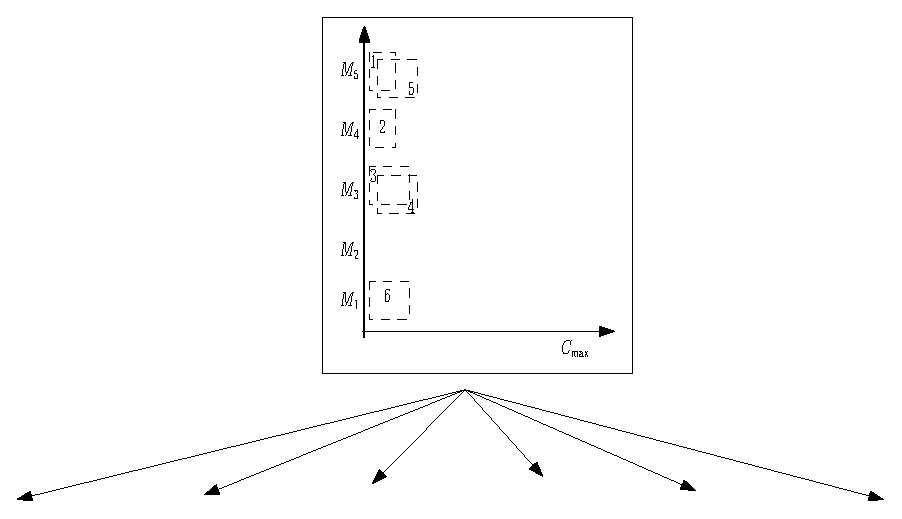
\includegraphics[width=0.7\textwidth]{game-1} \end{figure}        
	\end{example} 
	\begin{example}{Second layer -- all possible first dispatches at step $k=2$}
		\begin{figure} \centering 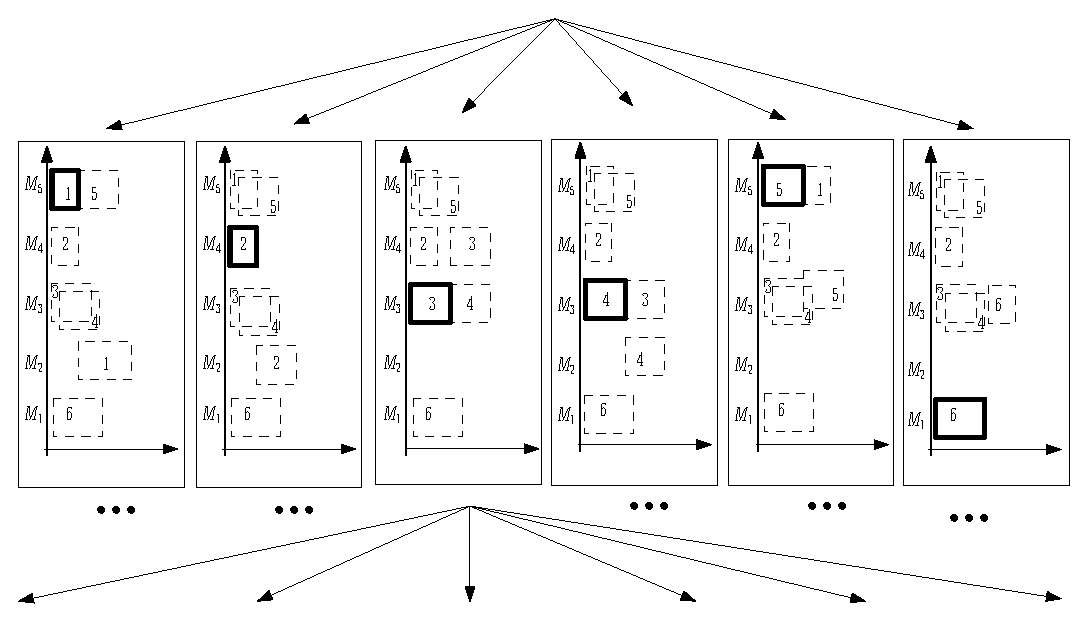
\includegraphics[width=0.7\textwidth]{game-2} \end{figure}        
	\end{example}
	\begin{example}{Third layer -- given $J_3$ is dispatched first on $M_3$ at step $k=3$}
		\begin{figure} \centering 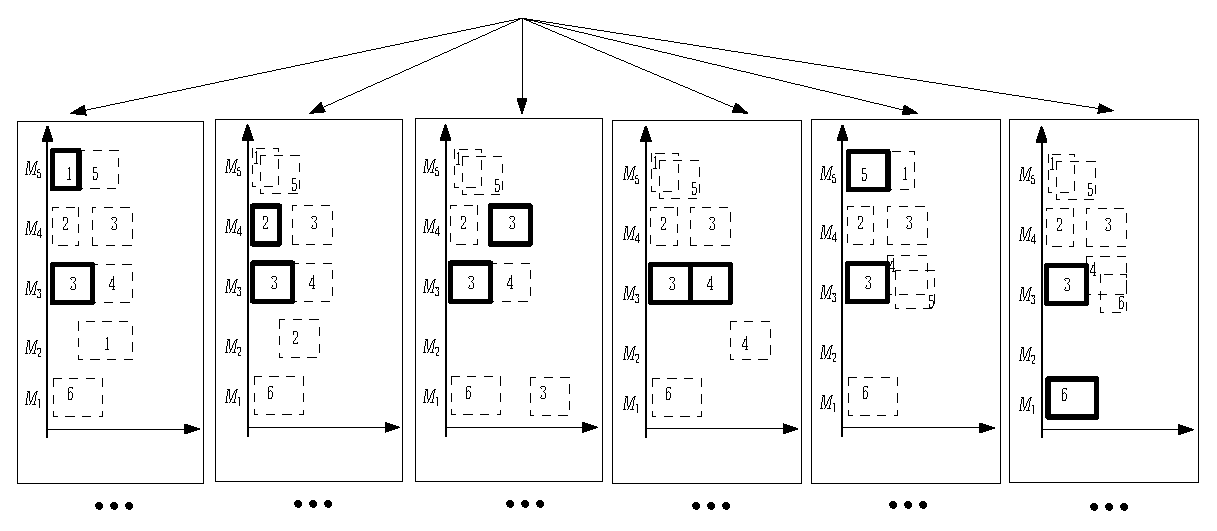
\includegraphics[width=0.7\textwidth]{game-3} \end{figure}        
	\end{example}
}


\section{Preference Learning}
\frame{\tableofcontents[currentsection]}

\frame[allowframebreaks]{\frametitle{Ordinal Regression}
	\begin{block}{Preference learning problem}
		Specified by a set of \alert{preference pairs}:
		\begin{equation*}
		S = \left\{\left\{\vec{z}_o,+1)\right\}_{k=1}^{\ell},\left\{\vec{z}_s,-1)\right\}_{k=1}^{\ell}
		\;|\;\forall o\in \mathcal{O}^{(k)},s\in \mathcal{S}^{(k)}
		\right\}\subset \Phi\times Y \label{eq:S}
		\end{equation*}
		where the set of point/rank pairs are:
		\bi Optimal decision: $\vec{z_o}=\vphi^{(o)}-\vphi^{(s)}$, ranked $+1$
		\item Suboptimal decision: $\vec{z_s}=\vphi^{(s)}-\vphi^{(o)}$, ranked $-1$		
		\ei
		and $\vphi_o,\vphi_s\in\Phi\subset\mathcal{F}$ are features from the collected training set $\Phi$.
	\end{block}
	\framebreak
	
	\bi Mapping of points to ranks: $ \{h(\cdot) : \Phi \mapsto Y\}$ where 
	\begin{equation}
	\vphi_o \succ \vphi_s \quad \Leftrightarrow \quad h(\vphi_o) > h(\vphi_s) \nonumber
	\end{equation}
	
	\item The preference is defined by a linear function, i.e. \alert{PREF model}:
	$$ h(\vphi) = \sum_{i=1}^d w_i \vphi = \inner{w}{\phi}. $$
	\item Logistic regression learns the optimal parameters $\vec{w}$ by solving:
	$$ \min_{\vec{w}}\quad \tfrac{1}{2}\inner{w}{w} + C \sum_{j=1}^{\abs{S}} \log\left(1 + e^{-y_j \inner{w}{z_j}}\right) $$ 
	\ei	
}

\frame[allowframebreaks]{\frametitle{Generating preference set $S$}
	\begin{block}{A seperate DR for each dispatch iteration}
		\bi At each dispatch  $k$ a number of data pairs are created
		\bi for each of the $N_{\text{train}}$ problem instance created. \ei 
		\item Deliberately create a separate data set for each dispatch  
		\bi Resulting in $\ell$ linear scheduling rules for solving a $n \times m$ JSP. \ei
		\ei 
	\end{block}
	Defining the size of the training set as $l'=\abs{\Phi}$, gives the size of the preference set as $\abs{S}=l=2l'$. 
	\bi If $l$ is too large, than sampling needs to be done. \ei 
	
	\begin{block}{Previous sampling approach  }
		The strategy was to follow some \alert{single optimal job} $j\in\mathcal{O}^{(k)}$, thus creating $\abs{\mathcal{O}^{(k)}}\cdot\abs{\mathcal{S}^{(k)}}$ feature pairs at each dispatch $k$, resulting in a training size of: 
		\begin{equation}
		l' = \sum_{q=1}^{N_{\text{train}}}\left(\sum_{k=1}^\ell \abs{\mathcal{O}^{(k)}}\cdot\abs{\mathcal{S}^{(k)}}\right) \nonumber
		\end{equation}
	\end{block}
	For the data distribution considered there, this simple sampling was sufficient for a favourable outcome. However for a considerably harder data distribution this strategy did not work well.
	
	% \begin{quote} Motivation: a brute force approach to investigate the feasibility of finding optimal weights $\vec{w}$.\end{quote} 
	
	\framebreak 
	\begin{block}{Trajectory sampling strategies explored for adding features to $\Phi$}
	\begin{description}
		\item[$\Phi^{opt}$] follow some (random) optimal task
		\item[$\Phi^{cma}$] follow the task corresponding to highest priority, computed with fixed weights $\vec{w}$, which were obtained by optimising with \beamergotobutton{CMA-ES}. 
		\item[$\Phi^{mwr}$] follow the SDR most work remaining (MWR).
		\item[$\Phi^{rnd}$] follow some random task.
		\item[$\Phi^{all}$] union of all of the above, i.e., 
		$$ \Phi^{all} = \Phi^{opt} \cup \Phi^{cma} \cup \Phi^{mwr} \cup \Phi^{rnd} $$
	\end{description}
	\end{block}
	
	\framebreak 
	\begin{block}{Ranking schemes implemented for adding preference pairs to $S$}
	\begin{itemize}
		\item[$S_{b}$] all opt rankings $r_1$ vs. all possible subopt rankings $r_i$, $i\in\{2,...,n'\}$
		\item[$S_{f}$] full subsequent rankings, i.e., all combinations of $r_i$ and $r_{i+1}$ for all $i\in\{1,...,n'\}$. 
		\item[$S_{p}$] partial subsequent rankings, similar ot $S_f$ except if there are more than one operation with the same ranking, only one is needed to be compared to subsequent rank, i.e., $S_p\subset S_f$.
		\item[$S_{a}$] union of all of the above, i.e., 
		$$ S_{a} = S_b \cup S_f \cup S_p$$
	\end{itemize}
	where $r_1>r_2>\cdots>r_{n'}$ $(n'\leq n)$ are the rankings of $\mathcal{R}^{(k)}$.
	\end{block}
}








\section{Evolutionary search with CMA-ES}
\frame{\tableofcontents[currentsection]}
\frame{\frametitle{Evolutionary search}\label{CMA-ES}
	Instead of using logistic regression for to find the weights $\vec{w}$ for linear preference function:
	$$ h(\vphi) = \sum_{i=1}^d w_i \vphi = \inner{w}{\vphi}. $$
	a widely-used evolutionary algorithm, Covariance Matrix Adaptation Evolution Strategy (\alert{CMA-ES}), is applied directly on the %desired 
	objective function. %For this study both,~~ \begin{enumerate*}[label=\itshape\alph*\upshape)]
	%\item expected relative error, \alert{$\mathbb{E}\left[\rho\right]$}; and
	%\item final makespan, \alert{$\mathbb{E}\left[C_{\max}\right]$}, 
	%\end{enumerate*} will be considered.
	
	\begin{description}\item[Benefit] No need to collect training data beforehand.
		\item[Drawback] Computationally expensive to evaluate $\mathbb{E}\left[C_{\max}\right]$
	\end{description}
}
\section{Experiments}
\frame{\tableofcontents[currentsection]}

\frame[allowframebreaks]{\frametitle{Experiments}
\begin{block}{Size of preference set, $l=|S|$}
\vspace{-12pt}
\begin{figure} \centering
\includegraphics[width=0.75\textwidth]{numTrainingData.pdf}
\end{figure}
\vspace{-12pt}
\end{block}
\framebreak
\begin{block}{Box-plot for PREF models using test set}
\vspace{-12pt}
\begin{figure} \centering
\includegraphics[width=0.62\textwidth]{boxplot.pdf}
\end{figure}
\vspace{-12pt}
\end{block}
\framebreak
\begin{block}{Trajectory sampling strategies}
\bi Learning preferences from good scheduling rules can give favourable results, e.g. $\Phi^{cma}$ and $\Phi^{mwr}$.
\item Tracking only optimal paths (\alert{$\Phi^{opt}$}) yield a generally lower mean relative error -- although there was no statistical difference with $\Phi^{rnd}$, implying the model has diverged from the learned optimal features set and is inept to determine good dispatches from that point onward.
\item For $\mathcal{P}_{j.rnd}^{6\times5}$ the best model was based on \alert{$\Phi^{all}$}, where the suboptimal trajectories aid $\Phi^{opt}$ by adding a greater variety of preference pairs for getting out of local minima.
\ei 
\end{block}
\begin{block}{Results for ranking schemes}
	\bi No statistical difference between ranking schemes. However, opting for a smaller preference set then \alert{$S_p$} is preferred. 
	\ei 
\end{block}
}

\section{Summary and conclusions}
\frame{\tableofcontents[currentsection]}

\frame[allowframebreaks]{\frametitle{Summary and conclusions}
\bi Introduced a framework for learning linear composite dispatch rules for scheduling. 
\item The approach is based on preference learning and its success is highly dependent on the preference pairs introduced to the system, i.e., the trajectories explored through the state-space. Here, optimal and suboptimal trajectories are of value.
\item By partial subsequent ranking scheme it's possible to reduce the preference set without loss of performance. 
\ei
\begin{block}{Future work}
\bi Instead of creating preference set based on collecting trajectories based on arbitrary dispatching rules (or models), it's worthwhile to continue with $PREF^{opt}$ model and collect preference set following its learned policy and use that to create a new model similar to $\Phi^{all}$. 
\item Namely use the model to update itself -- also known as \alert{imitation learning}.
\item 
Preliminary experiments have shown that a $PREF^{opt}$ with 14.07\% mean relative error can be improved to 8.52\% with only one unsupervised iteration, or 9.98\% if iteration is supervised.\footnote{Supervised set-up: 50\% chance $PREF^{opt}$ used, 50\% optimal move chosen.}
\ei
\end{block}
}

\frame{
\frametitle{Thank you for your attention}
\vspace{2cm}
\begin{center} \pause {\huge\bf Questions?} \end{center}
\vfill
\begin{flushright} Contact: Helga Ingimundard\'{o}ttir, \url{hei2@hi.is}\end{flushright}
}

\end{document}